\documentclass[tikz, border=5pt]{standalone}
\usetikzlibrary{perspective, arrows.meta}

\usepackage{bm}

\begin{document}

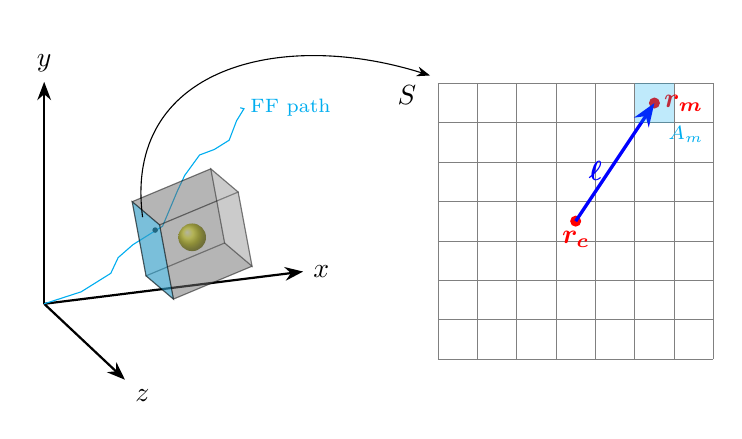
\begin{tikzpicture}[>=Stealth]
	\begin{scope}[3d view={70}{20}]
		% zxy (labels) is actually xyz (tikz cs)
		\draw[->, thick] (0, 0, 0) -- (3, 0, 0) node[below right] {$z$};
		\draw[->, thick] (0, 0, 0) -- (0, 3.5, 0) node[right] {$x$};
		\draw[->, thick] (0, 0, 0) -- (0, 0, 3) node[above] {$y$};

		\draw[cyan]
			(0, 0, 0)      -- (0, 0.5, 0.1)  -- (0, 0.7, 0.2)  --
			(0, 0.8, 0.25) -- (0, 0.9, 0.3)  -- (0, 1.0, 0.5)  --
			(0, 1.2, 0.65) -- (0, 1.3, 0.7)  -- (0, 1.4, 0.75) --
			(0, 1.6, 0.85) -- (0, 1.8, 1.3)  -- (0, 1.9, 1.5)  --
			(0, 2.1, 1.75) -- (0, 2.3, 1.8)  -- (0, 2.5, 1.9)  --
			(0, 2.6, 2.15) -- (0, 2.7, 2.3)  -- (0, 2.65, 2.32)
			node [very near end, right, font=\scriptsize] {FF path};

		\fill[black] (0, 1.5, 0.81) circle [radius=1pt];

		\shade[ball color=yellow]
			(0, 2.0, 0.65) circle [radius=5pt];
	\end{scope}

	\begin{scope}[
		rotate around x=0,
		rotate around y=40,
		rotate around z=10,
		shift={(1.9, 0.1)}
	]
		\coordinate (O) at (-0.5,-0.5,-0.5);
		\coordinate (A) at (0.5,-0.5,-0.5);
		\coordinate (B) at (0.5,0.5,-0.5);
		\coordinate (C) at (-0.5,0.5,-0.5);
		\coordinate (D) at (-0.5,-0.5,0.5);
		\coordinate (E) at (0.5,-0.5,0.5);
		\coordinate (F) at (0.5,0.5,0.5);
		\coordinate (G) at (-0.5,0.5,0.5);

		\filldraw[fill=black!80, opacity=0.3]
			(O) -- (A) -- (B) -- (C) -- cycle; % back
		\filldraw[fill=gray!80, opacity=0.3]
			(B) -- (C) -- (G) -- (F) -- cycle; % top
		\filldraw[fill=black!80, opacity=0.3]
			(O) -- (A) -- (E) -- (D) -- cycle; % bottom
		\filldraw[fill=gray!80, opacity=0.3]
			(D) -- (E) -- (F) -- (G) -- cycle; % front
		\filldraw[fill=gray!80, opacity=0.3]
			(A) -- (B) -- (F) -- (E) -- cycle; % left
		\filldraw[fill=cyan!80, opacity=0.5]
			(O) -- (C) -- (G) -- (D) -- cycle; % left
	\end{scope}

	\draw[->]
		(1.25, 1.1) .. controls (1, 3) and (3, 3.5) .. (4.9, 2.9)
		node [below right=5pt, very near end] {$S$};

	% surface mesh in detail
	\begin{scope}[xshift=5cm, yshift=-0.7cm]
		\coordinate (C) at (1.75, 1.75);
		\coordinate (M) at (2.75, 3.25);

		\draw[step=0.5cm, gray, very thin] (0, 0) grid (3.5, 3.5);

		\fill[red] (C) circle [radius=2pt] node [below] {$\bm{r_c}$};
		\fill[red] (M) circle [radius=2pt] node [right] {$\bm{r_m}$};

		\draw[->, blue, very thick] (C) --  node [near start, above] {$\bm{\ell}$} (M);

		\fill[cyan, nearly transparent] (2.5, 3.0) rectangle (3, 3.5);

		\path[font=\scriptsize] (3.15, 2.85) node [cyan] {$A_m$};
	\end{scope}

\end{tikzpicture}

\end{document}
